\chapter[Lecture 1]{}\label{lec1}

Solid State Physics $\to$ Story of dressed electrons.

Fundamental particles $\to$ Fermions [quarks, leptons, antiquarks and antileptons]

\smallskip
Quarks $\to$
\begin{center}
\begin{tabular}{lll}
up $(u)$ & charm $(c)$ & top $(t)$\\[3pt]
down $(d)$ & strange $(s)$ & bottom $(b)$ 
\end{tabular}
\end{center}

Leptons $\to$
\begin{center}
\begin{tabular}{lll}
electron ($e$) & muon $(\mu)$ & tau $(\tau)$\\[3pt]
electron neutrino $(\nu_{e})$ & muon neutrino $(\nu_{\mu})$ & tau neutrino $(\nu_{\tau})$
\end{tabular}
\end{center}
and Higg's boson $(H)$.
\begin{figure}[H]
\centering
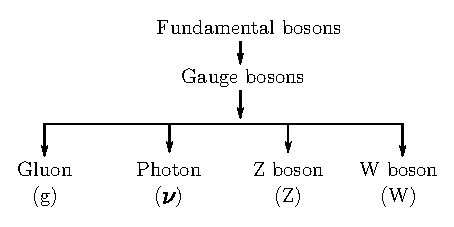
\includegraphics[scale=1.1]{images/lecture1/fig1.eps}
\end{figure}

These are force particles that mediate interactions between Fermions.

A particle containing two or more elementary particle is a composite particle.

Electron's three degrees of freedom {\em charge, spin, orbit} can separate via wave function into three quasiparticles holon, spinon, orbiton. However, a free electron - which is not orbiting around nucleus and has no orbital motion is unsplitable and remains regarded as an elementary particle.

\section*{Solid State Physics Course}

\textbf{Solid state physics -} A collection of ideas evolved over the time based on observations.

The questions often asked $\to$ what are the ideas those take us beyond the known paradigms ?

The most exotic phases people study in recent times.
\begin{itemize}
\item[(i)] Correlation Physics, Magnetism, Disorder

Spin excitations without charge

Spin liquid, Charge fractionalization 

Entanglement vs Pairing

\item[(ii)] Phase transitions, Quantum criticality $\to$ Confined/deconfined, criticality at T $\neq$ OK. Criticality.

\item[(iii)] Superconductivity, Superfluidity $\to$ Room temp. SC.

\item[(iv)] Quantum Hall effect $\to$ topological Insulators. 

Majorana Fermions

Weyl Semimetals

topological Quantum Computing
\end{itemize}
\begin{itemize}
\item[(a)] SSP provides a framework for describing and determining what happens to a large group of particles when they interact via (presumably) well-known forces.

\item[(b)] SSP deals with many interacting systems.

\item[(c)] Macroscopic properties are governed by Conservation laws and broken symmetry.

Particle no. is conserved.

High temp. $\to$ full translational + Rotational symmetry

Reduce temp. $\to$ New thermodynamically stable stats condense with progressively lowered symmetry.
\end{itemize}

\section*{Hydrogen Atom Problem}

The basis task is write down the Hamiltonian and then Schrodinger equation -
$$
H\psi = E\psi\qquad H = T+V
$$

$T=$ Kinetic energy

$V=$ Potential energy
$$
\therefore\quad H = -\dfrac{h^{2}\nabla^{2}}{2m}-\frac{1}{4\pi t_{0}}\dfrac{e^{2}}{r}
$$

\begin{figure}[H]
\centering
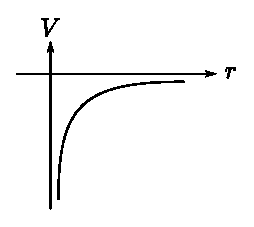
\includegraphics[scale=1.1]{images/lecture1/fig2.eps}
\end{figure}


To solve $\psi(r)=R(r)Y(\theta,\phi)$ use separation of variables method.

\smallskip

Radial Equation
$$
\dfrac{1}{R}\left[\dfrac{d}{dr}r^{2}\dfrac{dR}{dr}+\dfrac{2mr^{2}}{h^{2}}(E-V(r))R\right]=\lambda
$$

Angular Equation
\begin{gather*}
\dfrac{-\left(\dfrac{1}{\sin\theta}\dfrac{\partial}{\partial\theta}\sin\theta\dfrac{\partial}{\partial\theta}+\dfrac{1}{\sin^{2}\theta}\dfrac{\partial^{2}}{\partial\theta^{2}}\right)y(\theta,\phi)}{Y(\theta,\phi)}\\
a, \dfrac{\partial^{2}Y}{\partial \phi^{2}}=\sin\theta\dfrac{\partial}{\partial\theta}\sin\theta\dfrac{\partial Y}{\partial\theta}+\lambda\sin^{2}\theta Y
\end{gather*}

Again $Y=\Theta(\theta)\Phi (\phi)$
\begin{align*}
\psi_{nlm}(r,\theta,\phi) &= \sqrt{\left(\dfrac{2}{na^{*}_{0}}\right)^{3}\dfrac{(n-l-1)!}{2n(n+l)!}}e^{-\rho/2}\rho^{l}L^{2l+1}_{n-l-1}(\rho)Y^{m}_{l}(\theta,\phi)\\[4pt]
\rho &= \dfrac{2r}{na^{*}_{0}}\quad a^{*}_{0} = \text{reduced Bohr radius}\\[3pt]
&\hspace{1.8cm} = \dfrac{Y\pi\in 0 \hbar^{2}}{\mu l^{2}}
\end{align*}

$L$ $\to$ Generalized Laquerre Polynomial

\smallskip

$Y^{m}_{l}$ $\to$ Spherical harmonic function of degree $l$ and order $m$.
$$
Y_{lm}(\theta,\phi)=\sqrt{\dfrac{(2l+1)(l-m)!}{\pi(l+m)!}}
$$ 

$P_{lm}(\cos\theta)l^{im\phi}$ - Associated Legendre Polynomial.

Vector space sol$^{n}$
\begin{align*}
& \int |Y_{lm}(\theta,\phi)|^{2}d\Omega = 1\\[3pt]
& \int Y^{*}_{lm}Y_{l'm'}d\Omega=\delta_{ll'}\text{ (kronecker delta) } \delta_{mm'}
\end{align*}
Parity $\to P$
$$
P Y_{lm}(\theta,\phi)=Y(\pi-\theta,\phi+\pi)=(-1)^{l}Y_{lm}(\theta,\phi)
$$
$Y_{00}=\sqrt{\dfrac{1}{Y\pi}}$
\begin{align*}
Y_{11} &= -\sqrt{\dfrac{3}{8\pi}}\sin\theta e^{i\phi}\\[3pt]
Y_{10} &= -\sqrt{\dfrac{3}{4\pi}}\cos\theta\\[3pt]
Y_{1,-1} &= \sqrt{3}{8\pi}\sin\theta l^{-i\phi}
\end{align*}
\begin{align*}
Y_{2,-2} &= \sqrt{\dfrac{15}{32\pi}}\sin^{2}\theta e^{-2i\phi}\\[3pt]
Y_{2,-1} &= \sqrt{\dfrac{15}{8\pi}}\sin\theta \cos \theta l^{-i\phi}\\[3pt]
Y_{2,0} &= \sqrt{\dfrac{5}{16\pi}}(3\cos^{2}\theta-1)\\[3pt]
Y_{2,1} &= -\sqrt{\dfrac{15}{8\pi}}\sin \theta\cos \theta l^{i\phi}\\[3pt]
Y_{2,2} &= \sqrt{\dfrac{15}{32\pi}}\sin^{2}\theta l^{2i\pi}
\end{align*}
Radial Wave fns.
\begin{align*}
R_{10} &= \dfrac{1}{\sqrt{a^{3}}}l^{-\rho}\\[3pt]
R_{20} &= \dfrac{1}{\sqrt{2a^3}}\left(-1-\dfrac{\rho}{2}\right)l^{-\rho/2}\\[3pt]
R_{21} &= \dfrac{1}{2\sqrt{6a^3}}\rho e^{-\rho/2}\\[3pt]
R_{30} &= \dfrac{2}{3\sqrt{3a^{3}}}\left(1-\dfrac{2}{3}\rho +\dfrac{2}{27}\rho^{2}\right)e^{-\rho/3}\\[3pt]
R_{31} &= \dfrac{8}{27\sqrt{6a^{3}}}\rho \left(1-\rho/6\right)e^{-\rho/3}\\[3pt]
R_{32} &= \dfrac{4}{81\sqrt{30a^{3}}}\rho^{2}e^{-\rho/3}
\end{align*}
in Cartesian co-ordinate system -

\smallskip
E.g. $3d$ \ $n=3$, $l=0,1,2$ for $d$ \ $l=2$
\begin{longtable}{rl}
$\therefore\quad 3 d_{z^{2}} \simeq \psi_{320}$\hspace{1.62cm} & \raisebox{-1.1cm}{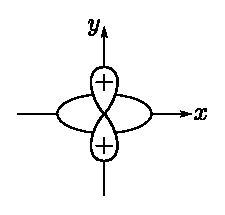
\includegraphics[scale=.8]{images/lecture1/fig3a.eps}}\\[1cm]
$3d_{n^{2}-y^{2}} \simeq \psi_{3,2,-2}+\psi_{3,2,2}$ & \raisebox{-1.1cm}{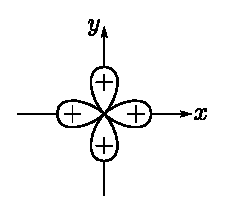
\includegraphics[scale=.8]{images/lecture1/fig3b.eps}}\\[1cm]
$3d_{xy} \simeq \psi_{3,2,-2}-\psi_{3,2,-2}$ & \raisebox{-1.1cm}{\includegraphics[scale=.8]{images/lecture1/fig3c.eps}}\\[1cm]
$3d_{xz} \simeq \psi_{3,2,1}+\psi_{3,2,-1}$ & \raisebox{-1.1cm}{\includegraphics[scale=.8]{images/lecture1/fig3d.eps}}\\[1cm]
$3d_{yz} \simeq \psi_{3,2,1}-\psi_{3,2,-1}$ & \raisebox{-1.1cm}{\includegraphics[scale=.8]{images/lecture1/fig3e.eps}}
\end{longtable}
\begin{figure}[H]
\centering
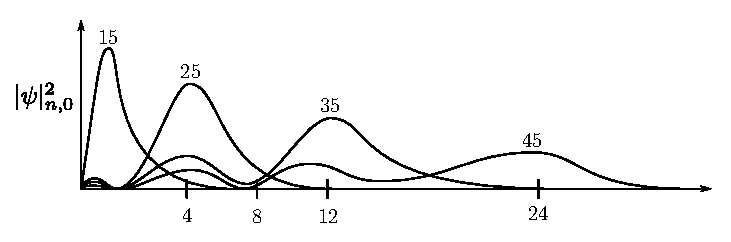
\includegraphics{images/lecture1/fig4a.eps}
\end{figure}
\begin{figure}[H]
\centering
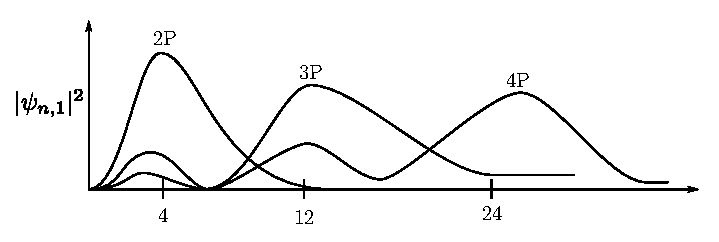
\includegraphics{images/lecture1/fig4b.eps}
\end{figure}
\begin{figure}[H]
\centering
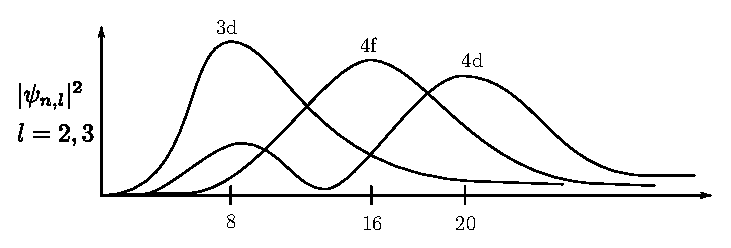
\includegraphics{images/lecture1/fig4c.eps}
\end{figure}

\newpage

{\bf H\boldmath$_{2}$O}

\begin{figure}[H]
\centering
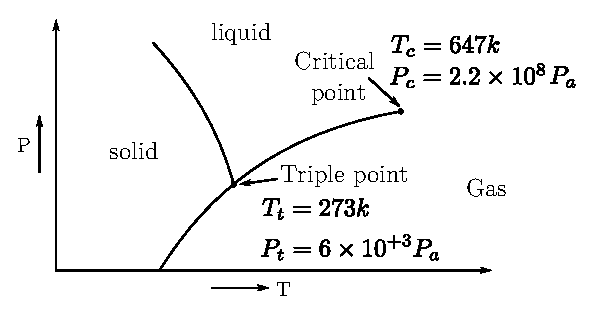
\includegraphics[scale=.9]{images/lecture1/fig5.eps}
\end{figure}
